
\documentclass[spanish, 11pt]{exam}

%These tell TeX which packages to use.
\usepackage{array,epsfig}
\usepackage{amsmath, textcomp}
\usepackage{amsfonts}
\usepackage{amssymb}
\usepackage{amsxtra}
\usepackage{amsthm}
\usepackage{mathrsfs}
\usepackage{color}
\usepackage{multicol, xparse}
\usepackage{verbatim}


\usepackage[utf8]{inputenc}
\usepackage[spanish]{babel}
\usepackage{eurosym}

\usepackage{graphicx}
\graphicspath{{../img/}}



\printanswers
\nopointsinmargin
\pointformat{}

%Pagination stuff.
%\setlength{\topmargin}{-.3 in}
%\setlength{\oddsidemargin}{0in}
%\setlength{\evensidemargin}{0in}
%\setlength{\textheight}{9.in}
%\setlength{\textwidth}{6.5in}
%\pagestyle{empty}

\let\multicolmulticols\multicols
\let\endmulticolmulticols\endmulticols
\RenewDocumentEnvironment{multicols}{mO{}}
 {%
  \ifnum#1=1
    #2%
  \else % More than 1 column
    \multicolmulticols{#1}[#2]
  \fi
 }
 {%
  \ifnum#1=1
  \else % More than 1 column
    \endmulticolmulticols
  \fi
 }
\renewcommand{\solutiontitle}{\noindent\textbf{Sol:}\enspace}

\newcommand{\samedir}{\mathbin{\!/\mkern-5mu/\!}}

\newcommand{\class}{4º ESO}
\newcommand{\examdate}{\today}

\newcommand{\tipo}{A}


\newcommand{\timelimit}{50 minutos}



\pagestyle{head}
\firstpageheader{
\includegraphics[width=0.2\columnwidth]{header_left}}{\textbf{Departamento de Matemáticas\linebreak \class}\linebreak \examnum}{
\includegraphics[width=0.1\columnwidth]{header_right}}
\runningheader{\class}{\examnum}{Página \thepage\ of \numpages}
\runningheadrule

\newcommand{\examnum}{Autoevaluación - Trimestre 3}
\begin{document}
\begin{questions}

%\question Representa y calcula las coordenadas de las siguientes combinaciones de $\overrightarrow{u}$ y $\overrightarrow{v}$:\begin{parts} \part[1] $2 \overrightarrow{u} - 3 \overrightarrow{v}$, $- 2 \overrightarrow{u}$, $- 2 \overrightarrow{u} - 2 \overrightarrow{v}$. Siendo $\overrightarrow{u}$ y $\overrightarrow{v}$: \\ \scalebox{.65}{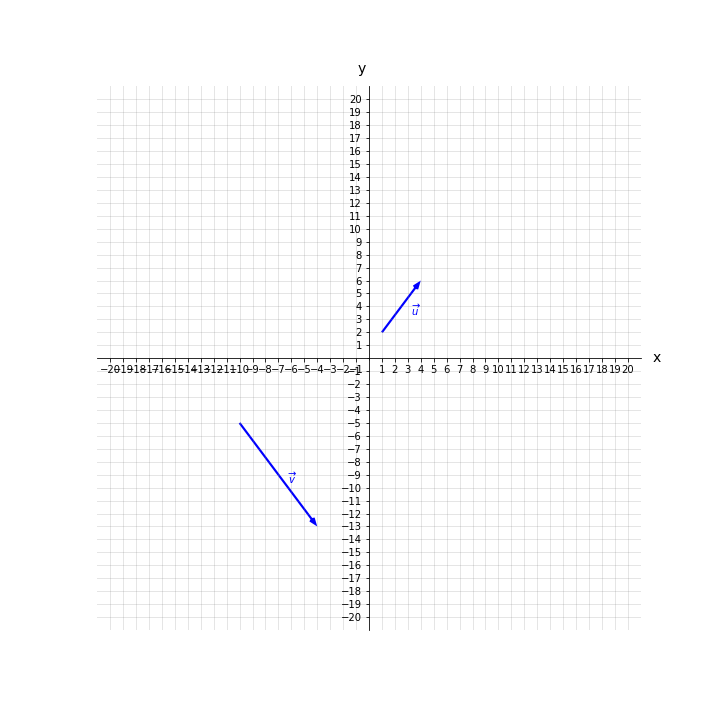
\includegraphics[width=1\columnwidth]{comb_vectores_0.png}}\begin{solution} $2 \overrightarrow{u} - 3 \overrightarrow{v}$, $- 2 \overrightarrow{u}$, $- 2 \overrightarrow{u} - 2 \overrightarrow{v}$\end{solution} \end{parts}


\question Representa y calcula las coordenadas de las siguientes combinaciones de $\overrightarrow{u}$ y $\overrightarrow{v}$: \begin{parts} \part[1] $\overrightarrow{u} + \overrightarrow{v}$, $\overrightarrow{u} + 2 \overrightarrow{v}$, $- 2 \overrightarrow{u}$. Siendo $\overrightarrow{u}$ y $\overrightarrow{v}$: \\\scalebox{.6}{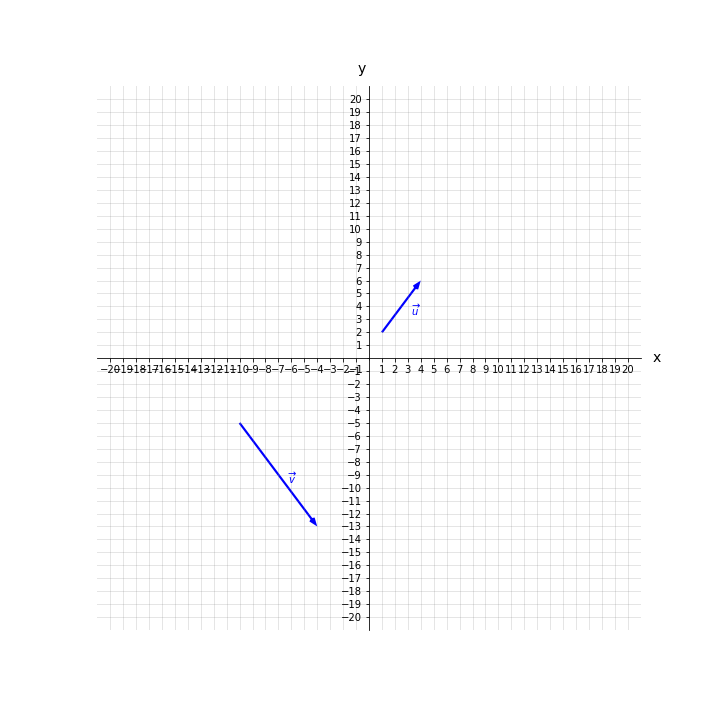
\includegraphics[width=1\columnwidth]{comb_lineal_0.png}} \\ \begin{solution} \scalebox{.63}{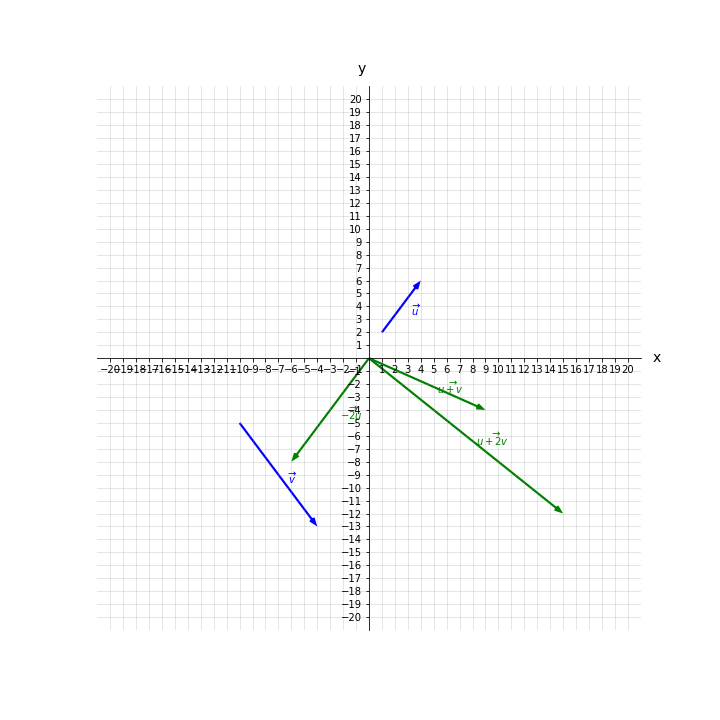
\includegraphics[width=1\columnwidth]{comb_lineal_sol_0.png}}\\ $Point2D\left(9, -4\right)$, $Point2D\left(15, -12\right)$, $Point2D\left(-6, -8\right)$\end{solution} \part[1] $\overrightarrow{u} + \overrightarrow{v}$, $\overrightarrow{u} - \overrightarrow{v}$, $\overrightarrow{u} + 2 \overrightarrow{v}$, $2 \overrightarrow{u} - \overrightarrow{v}$, $- 2 \overrightarrow{u}$. Siendo $\overrightarrow{u}$ y $\overrightarrow{v}$: \\\scalebox{.63}{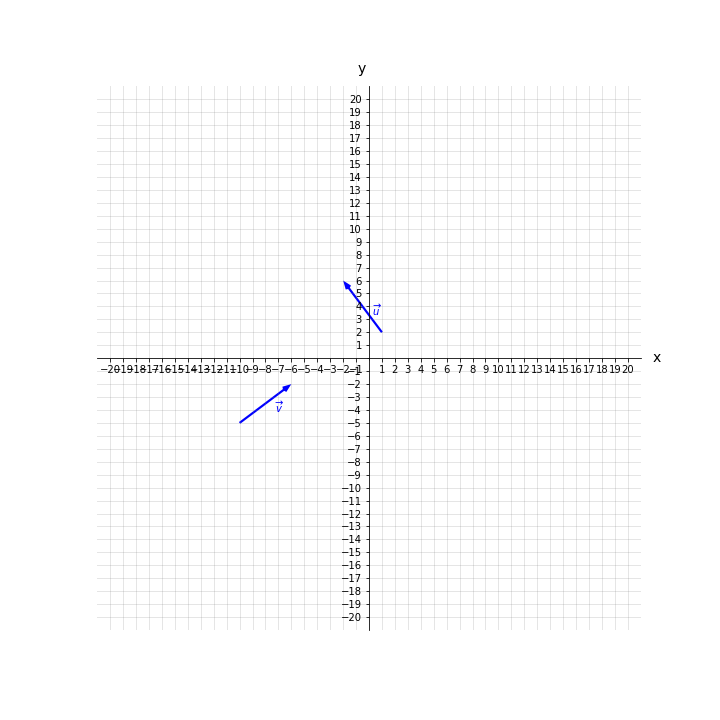
\includegraphics[width=1\columnwidth]{comb_lineal_1.png}} \\ \begin{solution} \scalebox{.65}{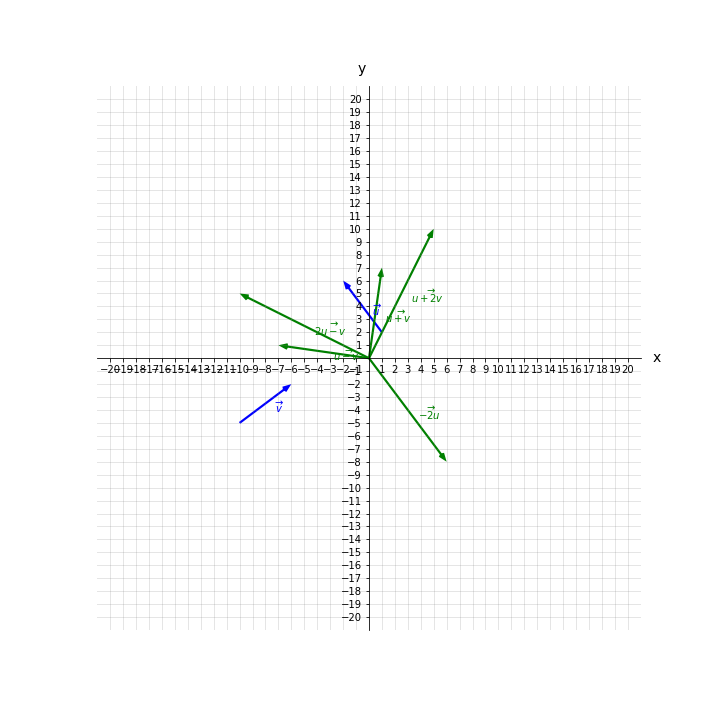
\includegraphics[width=1\columnwidth]{comb_lineal_sol_1.png}}\\ $Point2D\left(1, 7\right)$, $Point2D\left(-7, 1\right)$, $Point2D\left(5, 10\right)$, $Point2D\left(-10, 5\right)$, $Point2D\left(6, -8\right)$\end{solution} \end{parts} 

\question Calcula el punto medio del segmento que une los puntos:
\begin{multicols}{3}
\begin{parts} \part[1] $A\left( -5, \  1\right) y \ B\left( 3, \  7\right)$ \begin{solution} $M\left( -1, \  4\right)$\end{solution} \part[1] $A\left( 4, \  -1\right) y \ B\left( -2, \  -4\right)$ \begin{solution} $M\left( 1, \  - \frac{5}{2}\right)$\end{solution} \part[1] $A\left( 1, \  -5\right) y \ B\left( 5, \  -3\right)$ \begin{solution} $M\left( 3, \  -4\right)$\end{solution} \end{parts} 
\end{multicols}

\question Halla el valor de z para que los puntos A  , B    y C estén alineados. Siendo:
\begin{multicols}{3}
\begin{parts} \part[1] $A\left( 1, \  -2\right)$, $B \left( 3, \  1\right)$ y $C\left( 4, \  z\right)$ \begin{solution} $Point2D\left(2, 3\right)\parallel Point2D\left(3, z + 2\right) \to z=\left[ \frac{5}{2}\right]$\end{solution} \part[1] $A\left( 2, \  -4\right)$, $B \left( 5, \  3\right)$ y $C\left( 6, \  z\right)$ \begin{solution} $Point2D\left(3, 7\right)\parallel Point2D\left(4, z + 4\right) \to z=\left[ \frac{16}{3}\right]$\end{solution} \part[1] $A\left( 5, \  4\right)$, $B \left( -5, \  -2\right)$ y $C\left( 1, \  z\right)$ \begin{solution} $Point2D\left(-10, -6\right)\parallel Point2D\left(-4, z - 4\right) \to z=\left[ \frac{8}{5}\right]$\end{solution} \end{parts} 
\end{multicols}


\question Calcula el punto simétrico:
\begin{multicols}{2}
\begin{parts} \part[1] De $A\left( 7, \  6\right)$ respecto  de  $M\left( 2, \  1\right)$ \begin{solution} $Point2D\left(\dfrac{x}{2} + \dfrac{7}{2}, \dfrac{y}{2} + 3\right) = Point2D\left(2, 1\right)\to A'\left(-3,-4\right)$\end{solution} \part[1] De $A\left( 5, \  -3\right)$ respecto  de  $M\left( 1, \  3\right)$ \begin{solution} $Point2D\left(\dfrac{x}{2} + \dfrac{5}{2}, \dfrac{y}{2} - \dfrac{3}{2}\right) = Point2D\left(1, 3\right)\to A'\left(-3,9\right)$\end{solution} \part[1] De $A\left( 6, \  -5\right)$ respecto  de  $M\left( -3, \  2\right)$ \begin{solution} $Point2D\left(\dfrac{x}{2} + 3, \dfrac{y}{2} - \dfrac{5}{2}\right) = Point2D\left(-3, 2\right)\to A'\left(-12,9\right)$\end{solution} \part[1] De $A\left( -6, \  -2\right)$ respecto  de  $M\left( 4, \  1\right)$ \begin{solution} $Point2D\left(\dfrac{x}{2} - 3, \dfrac{y}{2} - 1\right) = Point2D\left(4, 1\right)\to A'\left(14,4\right)$\end{solution} \end{parts}
\end{multicols}

\end{questions}
\end{document}
